% Asset ID: FAS2PoissonDistributionTikZ-002
% Topic ID: FAS2PoissonDistribution
% Related lesson section: Section 8.7 and Section 9
% Source: FS1-Chp2-PoissonDistribution.pdf and transcripts.md
% Purpose: Cumulative probability and discrete inequality conversion visual.
\documentclass[tikz,border=8pt]{standalone}
\usepackage{amsmath}
\definecolor{Canvas}{HTML}{FAF9F6}
\definecolor{Panel}{HTML}{FFFFF0}
\definecolor{LineSoft}{HTML}{E5E5EA}
\definecolor{AccentGold}{HTML}{D4AF37}
\definecolor{TextInk}{HTML}{2C2C2E}
\definecolor{SoftPink}{HTML}{FBEFEF}
\definecolor{SoftGreen}{HTML}{DDEBC8}
\begin{document}
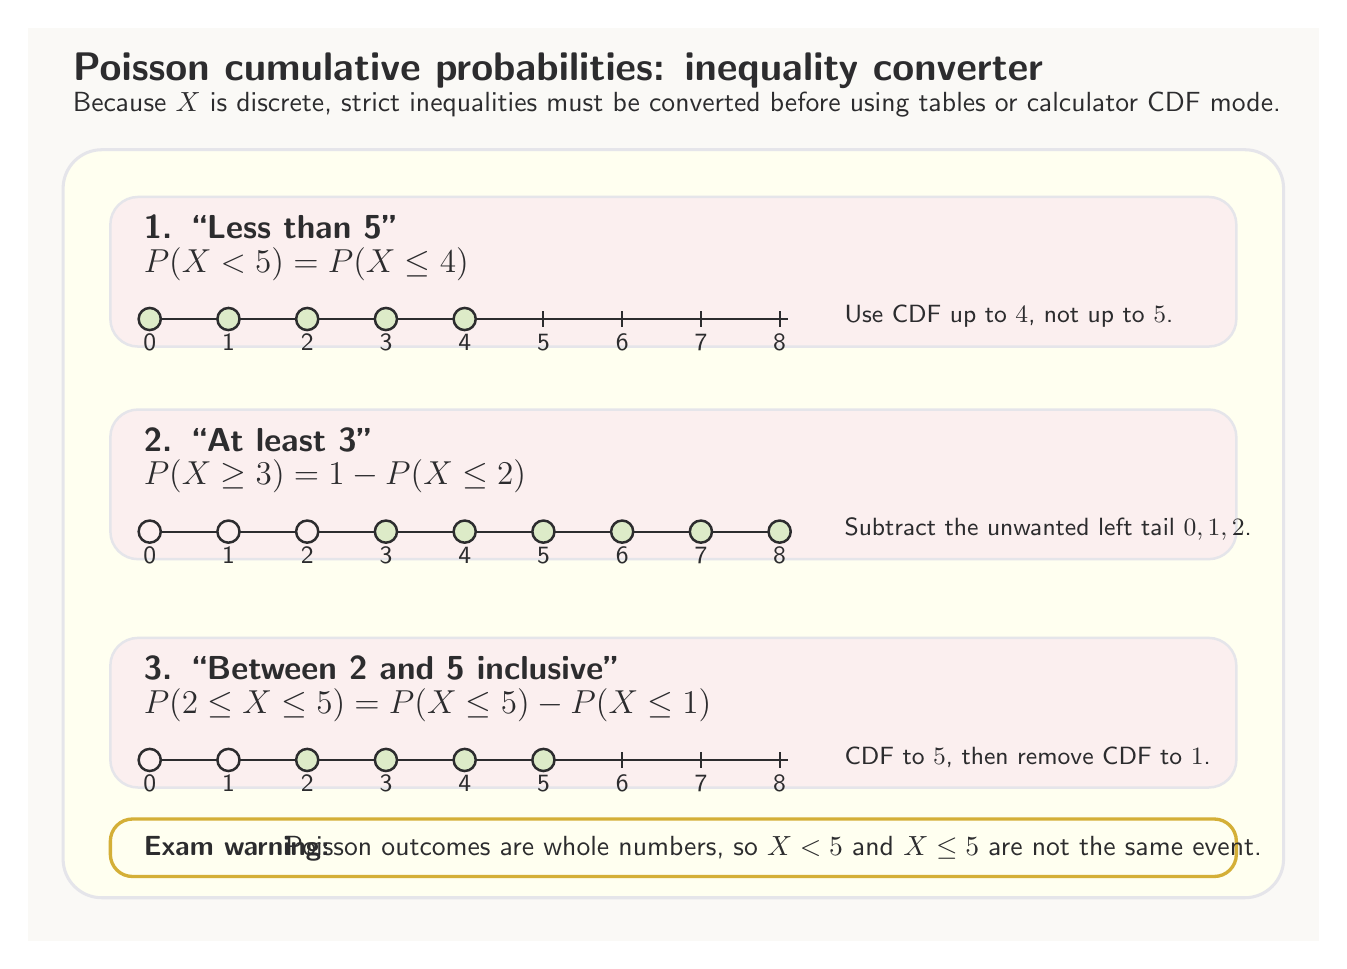
\begin{tikzpicture}[x=1cm,y=1cm,every node/.style={text=TextInk},dot/.style={circle,draw=TextInk,fill=Panel,line width=0.7pt,minimum size=6pt,inner sep=0pt},selected/.style={circle,draw=TextInk,fill=SoftGreen,line width=0.9pt,minimum size=8pt,inner sep=0pt},removed/.style={circle,draw=TextInk,fill=SoftPink,line width=0.9pt,minimum size=8pt,inner sep=0pt}]
\fill[Canvas] (-1,-1.2) rectangle (15.4,10.4);
\node[anchor=west,font=\sffamily\bfseries\Large] at (-0.55,9.85){Poisson cumulative probabilities: inequality converter};
\node[anchor=west,font=\sffamily\normalsize] at (-0.55,9.42){Because \(X\) is discrete, strict inequalities must be converted before using tables or calculator CDF mode.};
\draw[fill=Panel,draw=LineSoft,line width=1.1pt,rounded corners=14pt] (-0.55,-0.65) rectangle (14.95,8.85);
\foreach \y/\title/\formula/\note in {7.35/{1. ``Less than 5''}/{\(P(X<5)=P(X\leq4)\)}/{Use CDF up to \(4\), not up to \(5\).},4.65/{2. ``At least 3''}/{\(P(X\geq3)=1-P(X\leq2)\)}/{Subtract the unwanted left tail \(0,1,2\).},1.75/{3. ``Between 2 and 5 inclusive''}/{\(P(2\leq X\leq5)=P(X\leq5)-P(X\leq1)\)}/{CDF to \(5\), then remove CDF to \(1\).}}{
  \draw[fill=SoftPink,draw=LineSoft,line width=0.9pt,rounded corners=10pt] (0.05,\y-1) rectangle (14.35,\y+0.9);
  \node[anchor=west,font=\sffamily\bfseries\large] at (0.35,\y+0.52){\title};
  \node[anchor=west,font=\sffamily\large] at (0.35,\y+0.05){\formula};
  \draw[TextInk,line width=0.7pt] (0.55,\y-0.65) -- (8.65,\y-0.65);
  \foreach \x in {0,1,2,3,4,5,6,7,8}{\draw[TextInk,line width=0.7pt] ({0.55+\x},\y-0.75)--({0.55+\x},\y-0.55);\node[font=\sffamily\small] at ({0.55+\x},\y-0.95){\x};}
  \node[anchor=west,font=\sffamily\small,align=left] at (9.25,\y-0.62){\note};
}
\foreach \x in {0,1,2,3,4}{\node[selected] at ({0.55+\x},6.70){};}
\foreach \x in {0,1,2}{\node[removed] at ({0.55+\x},4.00){};}\foreach \x in {3,4,5,6,7,8}{\node[selected] at ({0.55+\x},4.00){};}
\foreach \x in {0,1}{\node[removed] at ({0.55+\x},1.10){};}\foreach \x in {2,3,4,5}{\node[selected] at ({0.55+\x},1.10){};}
\draw[fill=Panel,draw=AccentGold,line width=1.2pt,rounded corners=8pt] (0.05,-0.38) rectangle (14.35,0.35);
\node[anchor=west,font=\sffamily\bfseries\normalsize] at (0.35,-0.02){Exam warning:};
\node[anchor=west,font=\sffamily\normalsize] at (2.15,-0.02){Poisson outcomes are whole numbers, so \(X<5\) and \(X\leq5\) are not the same event.};
\end{tikzpicture}
\end{document}
